% Options for packages loaded elsewhere
\PassOptionsToPackage{unicode}{hyperref}
\PassOptionsToPackage{hyphens}{url}
\PassOptionsToPackage{dvipsnames,svgnames,x11names}{xcolor}
%
\documentclass[
  12pt,
  letterpaper,
  DIV=11,
  numbers=noendperiod]{scrreprt}

\usepackage{amsmath,amssymb}
\usepackage{iftex}
\ifPDFTeX
  \usepackage[T1]{fontenc}
  \usepackage[utf8]{inputenc}
  \usepackage{textcomp} % provide euro and other symbols
\else % if luatex or xetex
  \usepackage{unicode-math}
  \defaultfontfeatures{Scale=MatchLowercase}
  \defaultfontfeatures[\rmfamily]{Ligatures=TeX,Scale=1}
\fi
\usepackage{lmodern}
\ifPDFTeX\else  
    % xetex/luatex font selection
  \setmainfont[]{Times New Roman}
  \setsansfont[]{Arial}
  \setmonofont[]{Courier New}
\fi
% Use upquote if available, for straight quotes in verbatim environments
\IfFileExists{upquote.sty}{\usepackage{upquote}}{}
\IfFileExists{microtype.sty}{% use microtype if available
  \usepackage[]{microtype}
  \UseMicrotypeSet[protrusion]{basicmath} % disable protrusion for tt fonts
}{}
\makeatletter
\@ifundefined{KOMAClassName}{% if non-KOMA class
  \IfFileExists{parskip.sty}{%
    \usepackage{parskip}
  }{% else
    \setlength{\parindent}{0pt}
    \setlength{\parskip}{6pt plus 2pt minus 1pt}}
}{% if KOMA class
  \KOMAoptions{parskip=half}}
\makeatother
\usepackage{xcolor}
\setlength{\emergencystretch}{3em} % prevent overfull lines
\setcounter{secnumdepth}{5}
% Make \paragraph and \subparagraph free-standing
\ifx\paragraph\undefined\else
  \let\oldparagraph\paragraph
  \renewcommand{\paragraph}[1]{\oldparagraph{#1}\mbox{}}
\fi
\ifx\subparagraph\undefined\else
  \let\oldsubparagraph\subparagraph
  \renewcommand{\subparagraph}[1]{\oldsubparagraph{#1}\mbox{}}
\fi

\usepackage{color}
\usepackage{fancyvrb}
\newcommand{\VerbBar}{|}
\newcommand{\VERB}{\Verb[commandchars=\\\{\}]}
\DefineVerbatimEnvironment{Highlighting}{Verbatim}{commandchars=\\\{\}}
% Add ',fontsize=\small' for more characters per line
\usepackage{framed}
\definecolor{shadecolor}{RGB}{241,243,245}
\newenvironment{Shaded}{\begin{snugshade}}{\end{snugshade}}
\newcommand{\AlertTok}[1]{\textcolor[rgb]{0.68,0.00,0.00}{#1}}
\newcommand{\AnnotationTok}[1]{\textcolor[rgb]{0.37,0.37,0.37}{#1}}
\newcommand{\AttributeTok}[1]{\textcolor[rgb]{0.40,0.45,0.13}{#1}}
\newcommand{\BaseNTok}[1]{\textcolor[rgb]{0.68,0.00,0.00}{#1}}
\newcommand{\BuiltInTok}[1]{\textcolor[rgb]{0.00,0.23,0.31}{#1}}
\newcommand{\CharTok}[1]{\textcolor[rgb]{0.13,0.47,0.30}{#1}}
\newcommand{\CommentTok}[1]{\textcolor[rgb]{0.37,0.37,0.37}{#1}}
\newcommand{\CommentVarTok}[1]{\textcolor[rgb]{0.37,0.37,0.37}{\textit{#1}}}
\newcommand{\ConstantTok}[1]{\textcolor[rgb]{0.56,0.35,0.01}{#1}}
\newcommand{\ControlFlowTok}[1]{\textcolor[rgb]{0.00,0.23,0.31}{#1}}
\newcommand{\DataTypeTok}[1]{\textcolor[rgb]{0.68,0.00,0.00}{#1}}
\newcommand{\DecValTok}[1]{\textcolor[rgb]{0.68,0.00,0.00}{#1}}
\newcommand{\DocumentationTok}[1]{\textcolor[rgb]{0.37,0.37,0.37}{\textit{#1}}}
\newcommand{\ErrorTok}[1]{\textcolor[rgb]{0.68,0.00,0.00}{#1}}
\newcommand{\ExtensionTok}[1]{\textcolor[rgb]{0.00,0.23,0.31}{#1}}
\newcommand{\FloatTok}[1]{\textcolor[rgb]{0.68,0.00,0.00}{#1}}
\newcommand{\FunctionTok}[1]{\textcolor[rgb]{0.28,0.35,0.67}{#1}}
\newcommand{\ImportTok}[1]{\textcolor[rgb]{0.00,0.46,0.62}{#1}}
\newcommand{\InformationTok}[1]{\textcolor[rgb]{0.37,0.37,0.37}{#1}}
\newcommand{\KeywordTok}[1]{\textcolor[rgb]{0.00,0.23,0.31}{#1}}
\newcommand{\NormalTok}[1]{\textcolor[rgb]{0.00,0.23,0.31}{#1}}
\newcommand{\OperatorTok}[1]{\textcolor[rgb]{0.37,0.37,0.37}{#1}}
\newcommand{\OtherTok}[1]{\textcolor[rgb]{0.00,0.23,0.31}{#1}}
\newcommand{\PreprocessorTok}[1]{\textcolor[rgb]{0.68,0.00,0.00}{#1}}
\newcommand{\RegionMarkerTok}[1]{\textcolor[rgb]{0.00,0.23,0.31}{#1}}
\newcommand{\SpecialCharTok}[1]{\textcolor[rgb]{0.37,0.37,0.37}{#1}}
\newcommand{\SpecialStringTok}[1]{\textcolor[rgb]{0.13,0.47,0.30}{#1}}
\newcommand{\StringTok}[1]{\textcolor[rgb]{0.13,0.47,0.30}{#1}}
\newcommand{\VariableTok}[1]{\textcolor[rgb]{0.07,0.07,0.07}{#1}}
\newcommand{\VerbatimStringTok}[1]{\textcolor[rgb]{0.13,0.47,0.30}{#1}}
\newcommand{\WarningTok}[1]{\textcolor[rgb]{0.37,0.37,0.37}{\textit{#1}}}

\providecommand{\tightlist}{%
  \setlength{\itemsep}{0pt}\setlength{\parskip}{0pt}}\usepackage{longtable,booktabs,array}
\usepackage{calc} % for calculating minipage widths
% Correct order of tables after \paragraph or \subparagraph
\usepackage{etoolbox}
\makeatletter
\patchcmd\longtable{\par}{\if@noskipsec\mbox{}\fi\par}{}{}
\makeatother
% Allow footnotes in longtable head/foot
\IfFileExists{footnotehyper.sty}{\usepackage{footnotehyper}}{\usepackage{footnote}}
\makesavenoteenv{longtable}
\usepackage{graphicx}
\makeatletter
\def\maxwidth{\ifdim\Gin@nat@width>\linewidth\linewidth\else\Gin@nat@width\fi}
\def\maxheight{\ifdim\Gin@nat@height>\textheight\textheight\else\Gin@nat@height\fi}
\makeatother
% Scale images if necessary, so that they will not overflow the page
% margins by default, and it is still possible to overwrite the defaults
% using explicit options in \includegraphics[width, height, ...]{}
\setkeys{Gin}{width=\maxwidth,height=\maxheight,keepaspectratio}
% Set default figure placement to htbp
\makeatletter
\def\fps@figure{htbp}
\makeatother
\newlength{\cslhangindent}
\setlength{\cslhangindent}{1.5em}
\newlength{\csllabelwidth}
\setlength{\csllabelwidth}{3em}
\newlength{\cslentryspacingunit} % times entry-spacing
\setlength{\cslentryspacingunit}{\parskip}
\newenvironment{CSLReferences}[2] % #1 hanging-ident, #2 entry spacing
 {% don't indent paragraphs
  \setlength{\parindent}{0pt}
  % turn on hanging indent if param 1 is 1
  \ifodd #1
  \let\oldpar\par
  \def\par{\hangindent=\cslhangindent\oldpar}
  \fi
  % set entry spacing
  \setlength{\parskip}{#2\cslentryspacingunit}
 }%
 {}
\usepackage{calc}
\newcommand{\CSLBlock}[1]{#1\hfill\break}
\newcommand{\CSLLeftMargin}[1]{\parbox[t]{\csllabelwidth}{#1}}
\newcommand{\CSLRightInline}[1]{\parbox[t]{\linewidth - \csllabelwidth}{#1}\break}
\newcommand{\CSLIndent}[1]{\hspace{\cslhangindent}#1}

\usepackage{lipsum}
\usepackage{setspace}
\onehalfspacing
\linespread{1.5}
\KOMAoption{captions}{tableheading}
\makeatletter
\makeatother
\makeatletter
\@ifpackageloaded{bookmark}{}{\usepackage{bookmark}}
\makeatother
\makeatletter
\@ifpackageloaded{caption}{}{\usepackage{caption}}
\AtBeginDocument{%
\ifdefined\contentsname
  \renewcommand*\contentsname{Table of contents}
\else
  \newcommand\contentsname{Table of contents}
\fi
\ifdefined\listfigurename
  \renewcommand*\listfigurename{List of Figures}
\else
  \newcommand\listfigurename{List of Figures}
\fi
\ifdefined\listtablename
  \renewcommand*\listtablename{List of Tables}
\else
  \newcommand\listtablename{List of Tables}
\fi
\ifdefined\figurename
  \renewcommand*\figurename{Figure}
\else
  \newcommand\figurename{Figure}
\fi
\ifdefined\tablename
  \renewcommand*\tablename{Table}
\else
  \newcommand\tablename{Table}
\fi
}
\@ifpackageloaded{float}{}{\usepackage{float}}
\floatstyle{ruled}
\@ifundefined{c@chapter}{\newfloat{codelisting}{h}{lop}}{\newfloat{codelisting}{h}{lop}[chapter]}
\floatname{codelisting}{Listing}
\newcommand*\listoflistings{\listof{codelisting}{List of Listings}}
\makeatother
\makeatletter
\@ifpackageloaded{caption}{}{\usepackage{caption}}
\@ifpackageloaded{subcaption}{}{\usepackage{subcaption}}
\makeatother
\makeatletter
\@ifpackageloaded{tcolorbox}{}{\usepackage[skins,breakable]{tcolorbox}}
\makeatother
\makeatletter
\@ifundefined{shadecolor}{\definecolor{shadecolor}{rgb}{.97, .97, .97}}
\makeatother
\makeatletter
\makeatother
\makeatletter
\makeatother
\ifLuaTeX
  \usepackage{selnolig}  % disable illegal ligatures
\fi
\IfFileExists{bookmark.sty}{\usepackage{bookmark}}{\usepackage{hyperref}}
\IfFileExists{xurl.sty}{\usepackage{xurl}}{} % add URL line breaks if available
\urlstyle{same} % disable monospaced font for URLs
\hypersetup{
  pdftitle={How ecological interactions shape microbial mutation rates},
  pdfauthor={Rowan Green},
  colorlinks=true,
  linkcolor={blue},
  filecolor={Maroon},
  citecolor={Blue},
  urlcolor={Blue},
  pdfcreator={LaTeX via pandoc}}

\title{How ecological interactions shape microbial mutation rates}
\usepackage{etoolbox}
\makeatletter
\providecommand{\subtitle}[1]{% add subtitle to \maketitle
  \apptocmd{\@title}{\par {\large #1 \par}}{}{}
}
\makeatother
\subtitle{A thesis submitted to the University of Manchester for the
degree of Doctor of Philosophy in the Faculty of Science and
Engineering.}
\author{Rowan Green}
\date{2024}

\begin{document}
\maketitle
\ifdefined\Shaded\renewenvironment{Shaded}{\begin{tcolorbox}[interior hidden, borderline west={3pt}{0pt}{shadecolor}, frame hidden, breakable, enhanced, boxrule=0pt, sharp corners]}{\end{tcolorbox}}\fi

\renewcommand*\contentsname{Table of contents}
{
\hypersetup{linkcolor=}
\setcounter{tocdepth}{2}
\tableofcontents
}
\listoffigures
\listoftables
\bookmarksetup{startatroot}

\hypertarget{preface}{%
\chapter*{Preface}\label{preface}}
\addcontentsline{toc}{chapter}{Preface}

\markboth{Preface}{Preface}

This is a Quarto book.

To learn more about Quarto books visit
\url{https://quarto.org/docs/books}.

Mutagenesis is responsive to many environmental factors. Evolution
therefore depends on the environment not only for selection but also in
determining the variation available in a population. One such
environmental dependency is the inverse relationship between mutation
rates and population density in many microbial species. Here we
determine the mechanism responsible for this mutation rate plasticity.
Using dynamical computational modelling and in vivo mutation rate
estimation we show that the negative relationship between mutation rate
and population density arises from the collective ability of microbial
populations to control concentrations of hydrogen peroxide. We
demonstrate a loss of this density-associated mutation rate plasticity
when Escherichia coli populations are deficient in the degradation of
hydrogen peroxide. We further show that the reduction in mutation rate
in denser populations is restored in peroxide degradation-deficient
cells by the presence of wild-type cells in a mixed population.
Together, these model-guided experiments provide a mechanistic
explanation for density-associated mutation rate plasticity, applicable
across all domains of life, and frames mutation rate as a dynamic trait
shaped by microbial community composition.

\bookmarksetup{startatroot}

\hypertarget{introduction}{%
\chapter{Introduction}\label{introduction}}

Uncovering the mechanisms behind environmentally responsive mutagenesis
informs our understanding of evolution, notably antimicrobial
resistance, where mutation supply can be critical (Gifford et al. 2023;
Ragheb et al. 2019). Microbial mutation rates are responsive to a wide
variety of environmental factors including population density (Krašovec
et al. 2017), temperature (Chu et al. 2018), growth rate (Maharjan and
Ferenci 2018; Liu and Zhang 2019), stress (MacLean, Torres-Barceló, and
Moxon 2013; Foster 2007), growth phase (Loewe, Textor, and Scherer 2003)
and nutritional state (Maharjan and Ferenci 2017). Such mutation rate
plasticity inspires the idea of ``anti-evolution drugs'', able to slow
the evolution of antimicrobial resistance during the treatment of an
infection (Ragheb et al. 2019; Cirz et al. 2005; Domenech et al. 2020;
Alam et al. 2016). Even small reductions in the mutation rate (2-5-fold)
can have dramatic effects on the capacity of bacterial populations to
adapt to antibiotic treatment, particularly when evolution is limited by
mutation supply, as is the case for small pathogen populations (Ragheb
et al. 2019).

Microbial mutation rates have an inverse association with population
density across all domains of life, we have previously shown that 93\%
of otherwise unexplained variation in published mutation rate estimates
is explained by the final population density (Krašovec et al. 2017).
This density-associated mutation rate plasticity (DAMP) is a distinct
phenotype from stress-induced mutagenesis, which acts via independent
genetic mechanisms (Krašovec et al. 2018). Population density alters not
only the rate but also the spectrum of mutations, with significantly
higher rates of AT\textgreater GC transitions seen in low density
populations (Gifford et al. 2023). Density effects are likely relevant
to natural populations given that population sizes and densities vary
greatly, for example, \emph{Escherichia coli} populations in host faeces
can range in density by 5 orders of magnitude
(\href{https://www.biorxiv.org/content/10.1101/2023.09.27.557722v1.full\#ref-16}{\textbf{16}}),
and infections can be established by populations as small as
6×10\textsuperscript{3} cells
(\href{https://www.biorxiv.org/content/10.1101/2023.09.27.557722v1.full\#ref-17}{\textbf{17}}).
We therefore aim to mechanistically describe the widespread phenotype of
DAMP.

In order to test potential mechanisms generating DAMP, we developed and
systematically assessed a computational model connecting metabolism and
mutagenesis in a growing \emph{E. coli} population. This model generates
the hypothesis that the key determinants of DAMP are the production and
degradation rates of reactive oxygen species (ROS). Though molecular
oxygen is relatively stable it can be reduced to superoxide
(\textsuperscript{•}O\textsubscript{2−}), hydrogen peroxide
(H\textsubscript{2}O\textsubscript{2}) and hydroxyl radicals
(HO\textsuperscript{•}). These ``reactive oxygen species'' are strong
oxidants able to damage multiple biological molecules including
nucleotides and DNA
(\href{https://www.biorxiv.org/content/10.1101/2023.09.27.557722v1.full\#ref-18}{\textbf{18}}).
We tested the role of ROS in controlling DAMP by estimating mutation
rate plasticity under different conditions of environmental oxygen and
with genetic manipulations known to alter ROS dynamics. We find that the
reduction in mutation rate at increased population density results from
the population's increased ability to degrade
H\textsubscript{2}O\textsubscript{2}, resulting in reduced
ROS-associated mutagenesis. We show that this density effect is also
experienced by cells deficient in H\textsubscript{2}O\textsubscript{2}
degradation when cocultured with wild-type cells able to detoxify the
environment. Mutation rates therefore depend not only on the genotype of
the individual but also on the community's capacity to degrade
H\textsubscript{2}O\textsubscript{2}.

\bookmarksetup{startatroot}

\hypertarget{results}{%
\chapter{Results}\label{results}}

The results show mutations.

\bookmarksetup{startatroot}

\hypertarget{summary}{%
\chapter{Summary}\label{summary}}

In summary, this book has no content whatsoever.

\begin{Shaded}
\begin{Highlighting}[]
\DecValTok{1} \SpecialCharTok{+} \DecValTok{1}
\end{Highlighting}
\end{Shaded}

\begin{verbatim}
[1] 2
\end{verbatim}

\begin{Shaded}
\begin{Highlighting}[]
\FunctionTok{plot}\NormalTok{(}\FunctionTok{c}\NormalTok{(}\DecValTok{1}\SpecialCharTok{:}\DecValTok{3}\NormalTok{)}\SpecialCharTok{\textasciitilde{}}\FunctionTok{c}\NormalTok{(}\DecValTok{4}\SpecialCharTok{:}\DecValTok{6}\NormalTok{))}
\end{Highlighting}
\end{Shaded}

\begin{figure}[H]

{\centering 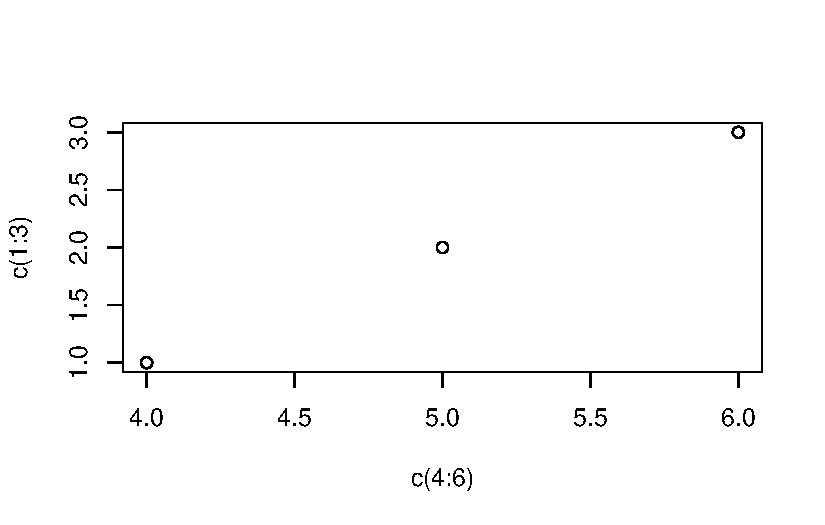
\includegraphics{summary_files/figure-pdf/fig-plot-1.pdf}

}

\caption{\label{fig-plot}Plot of numbers}

\end{figure}

\bookmarksetup{startatroot}

\hypertarget{references}{%
\chapter*{References}\label{references}}
\addcontentsline{toc}{chapter}{References}

\markboth{References}{References}

\hypertarget{refs}{}
\begin{CSLReferences}{1}{0}
\leavevmode\vadjust pre{\hypertarget{ref-Alam2016}{}}%
Alam, Md~Kausar, Areej Alhhazmi, John~F. DeCoteau, Yu Luo, and C.~Ronald
Geyer. 2016. {``RecA Inhibitors Potentiate Antibiotic Activity and Block
Evolution of Antibiotic Resistance.''} \emph{Cell Chemical Biology} 23
(3): 381--91. \url{https://doi.org/10.1016/j.chembiol.2016.02.010}.

\leavevmode\vadjust pre{\hypertarget{ref-Chu2018}{}}%
Chu, Xiao-Lin, Bo-Wen Zhang, Quan-Guo Zhang, Bi-Ru Zhu, Kui Lin, and
Da-Yong Zhang. 2018. {``Temperature Responses of Mutation Rate and
Mutational Spectrum in an Escherichia Coli Strain and the Correlation
with Metabolic Rate.''} \emph{BMC Evolutionary Biology} 18 (1).
\url{https://doi.org/10.1186/s12862-018-1252-8}.

\leavevmode\vadjust pre{\hypertarget{ref-Cirz2005}{}}%
Cirz, Ryan T, Jodie K Chin, David R Andes, Valérie de Crécy-Lagard,
William A Craig, and Floyd E Romesberg. 2005. {``Inhibition of Mutation
and Combating the Evolution of Antibiotic Resistance.''} Edited by Matt
Waldor. \emph{PLoS Biology} 3 (6): e176.
\url{https://doi.org/10.1371/journal.pbio.0030176}.

\leavevmode\vadjust pre{\hypertarget{ref-Domenech2020}{}}%
Domenech, Arnau, Ana Rita Brochado, Vicky Sender, Karina Hentrich,
Birgitta Henriques-Normark, Athanasios Typas, and Jan-Willem Veening.
2020. {``Proton Motive Force Disruptors Block Bacterial Competence and
Horizontal Gene Transfer.''} \emph{Cell Host \& Microbe} 27 (4):
544--555.e3. \url{https://doi.org/10.1016/j.chom.2020.02.002}.

\leavevmode\vadjust pre{\hypertarget{ref-Foster2007}{}}%
Foster, Patricia L. 2007. {``Stress-Induced Mutagenesis in Bacteria.''}
\emph{Critical Reviews in Biochemistry and Molecular Biology} 42 (5):
373--97. \url{https://doi.org/10.1080/10409230701648494}.

\leavevmode\vadjust pre{\hypertarget{ref-Gifford2023}{}}%
Gifford, Danna R., Anish Bhattacharyya, Alexandra Geim, Rok Marshall
Eleanor andKrašovec, and Christopher G. Knight. 2023. {``Environmental
and Genetic Influence on Rate and Spectrum of Spontaneous Mutations in
Escherichia Coli.''} \emph{biorXiv}, June.
\url{https://doi.org/10.1101/2023.04.06.535897}.

\leavevmode\vadjust pre{\hypertarget{ref-Krasovec2018}{}}%
Krašovec, Rok, Huw Richards, Danna R. Gifford, Roman V. Belavkin,
Alastair Channon, Elizabeth Aston, Andrew J. McBain, and Christopher G.
Knight. 2018. {``Opposing Effects of Final Population Density and Stress
on Escherichia Coli Mutation Rate.''} \emph{The ISME Journal} 12 (12):
2981--87. \url{https://doi.org/10.1038/s41396-018-0237-3}.

\leavevmode\vadjust pre{\hypertarget{ref-Krasovec2017}{}}%
Krašovec, Rok, Huw Richards, Danna R. Gifford, Charlie Hatcher, Katy J.
Faulkner, Roman V. Belavkin, Alastair Channon, Elizabeth Aston, Andrew
J. McBain, and Christopher G. Knight. 2017. {``Spontaneous Mutation Rate
Is a Plastic Trait Associated with Population Density Across Domains of
Life.''} Edited by Jeff Gore. \emph{PLOS Biology} 15 (8): e2002731.
\url{https://doi.org/10.1371/journal.pbio.2002731}.

\leavevmode\vadjust pre{\hypertarget{ref-Liu2019}{}}%
Liu, Haoxuan, and Jianzhi Zhang. 2019. {``Yeast Spontaneous Mutation
Rate and Spectrum Vary with Environment.''} \emph{Current Biology} 29
(10): 1584--1591.e3. \url{https://doi.org/10.1016/j.cub.2019.03.054}.

\leavevmode\vadjust pre{\hypertarget{ref-Loewe2003}{}}%
Loewe, Laurence, Volker Textor, and Siegfried Scherer. 2003. {``High
Deleterious Genomic Mutation Rate in Stationary Phase of
{\emph{Escherichia Coli}}.''} \emph{Science} 302 (5650): 1558--60.
\url{https://doi.org/10.1126/science.1087911}.

\leavevmode\vadjust pre{\hypertarget{ref-MacLean2013}{}}%
MacLean, R. Craig, Clara Torres-Barceló, and Richard Moxon. 2013.
{``Evaluating Evolutionary Models of Stress-Induced Mutagenesis in
Bacteria.''} \emph{Nature Reviews Genetics} 14 (3): 221--27.
\url{https://doi.org/10.1038/nrg3415}.

\leavevmode\vadjust pre{\hypertarget{ref-Maharjan2017}{}}%
Maharjan, Ram P., and Thomas Ferenci. 2017. {``A Shifting Mutational
Landscape in 6 Nutritional States: Stress-Induced Mutagenesis as a
Series of Distinct Stress Input{\textendash}mutation Output
Relationships.''} Edited by Jeff Gore. \emph{PLOS Biology} 15 (6):
e2001477. \url{https://doi.org/10.1371/journal.pbio.2001477}.

\leavevmode\vadjust pre{\hypertarget{ref-Maharjan2018}{}}%
---------. 2018. {``The Impact of Growth Rate and Environmental Factors
on Mutation Rates and Spectra in {\emph{Escherichia Coli}}.''}
\emph{Environmental Microbiology Reports} 10 (6): 626--33.
\url{https://doi.org/10.1111/1758-2229.12661}.

\leavevmode\vadjust pre{\hypertarget{ref-Ragheb2019}{}}%
Ragheb, Mark N., Maureen K. Thomason, Chris Hsu, Patrick Nugent, John
Gage, Ariana N. Samadpour, Ankunda Kariisa, et al. 2019. {``Inhibiting
the Evolution of Antibiotic Resistance.''} \emph{Molecular Cell} 73 (1):
157--165.e5. \url{https://doi.org/10.1016/j.molcel.2018.10.015}.

\end{CSLReferences}



\end{document}
